\documentclass[10pt, t]{beamer}

\newcommand\hmmax{0}
\newcommand\bmmax{0}

\usepackage[utf8]{inputenc}
\usepackage[T1]{fontenc}
\usepackage[usenames,dvipsnames,cmyk]{xcolor}
\usepackage[utopia]{mathdesign}
\usepackage[style=numeric-comp, 
            backend=biber,
            url=false,
            doi=true,
            eprint=false]{biblatex}
\usepackage{subcaption}
\usepackage{graphicx}
\usepackage{relsize}
% \usepackage{apacite}
\usepackage{amsmath}
\usepackage{amssymb}
\usepackage{mathtools}
\usepackage{siunitx}
\usepackage{braket}
\usepackage{physics}
\usepackage{tikz}
\usepackage{bm}
\usepackage{multirow}
\usepackage{animate}
% \usepackage{xmpmulti}

\setbeamercolor{}{fg=black, bg=white}
\setbeamercolor{frametitle}{fg=orange, bg=red!10}
\setbeamercolor{progress bar}{fg=red, bg=red!30}
\setbeamercolor{progress bar in head/foot}{fg=red, bg=red!30}
\setbeamercolor{progress bar in section page}{fg=red, bg=red!30}
\setbeamercolor{background canvas}{bg=white}

\definecolor{filecolor}{RGB}{180,43,190}
\definecolor{funccolor}{RGB}{150,83,210}
\newcommand{\hltexttt}[1]{\texttt{\color{filecolor}{#1}}}
\newcommand{\hltextttf}[1]{\texttt{\color{funccolor}{#1}}}
  
\usetikzlibrary{arrows.meta, shadows, shapes, arrows}

\addbibresource{text/refs.bib}

\usetheme[progressbar=frametitle]{metropolis}
\usepackage{appendixnumberbeamer}

\usepackage{booktabs}
\usepackage[scale=2]{ccicons}

\usepackage{pgfplots}
\usepgfplotslibrary{dateplot}

\usepackage{xspace}
\newcommand{\themename}{\textbf{\textsc{metropolis}}\xspace}

\newcommand{\onefigure}[1]{
    \begin{figure}[H]
        \centering
        \includegraphics[scale=0.28]{{#1}}
    \end{figure}
    \justifying
} %one figure {filename}{caption}
\newcommand{\twofigure}[2]{
    \begin{figure}[H]
        \centering
        \begin{subfigure}[b!]{0.49\textwidth}
            \centering
            \includegraphics[width=\textwidth]{{#1}}
        \end{subfigure}
        \begin{subfigure}[b!]{0.49\textwidth}
            \centering
            \includegraphics[width=\textwidth]{{#2}}
        \end{subfigure}
        \justify
    \end{figure}
} %two figure one-line {title}{file1}{caption1}{file2}{caption2}

\makeatletter
\newcolumntype{"}{@{\hskip\tabcolsep\vrule width 1.1pt\hskip\tabcolsep}}
\makeatother

\title{Quantum Many-Body Simulations of Double Dot System}
% \date{\today}
\date{}
\author{Alocias Mariadason}
\institute{}
% \titlegraphic{\hfill\includegraphics[height=1.5cm]{logo.pdf}}

\newcommand{\prtl}{\mathrm{\partial}} %reduce length of partial (less to write)
\NewDocumentCommand{\prd}{m O{} O{}}{\frac{\prtl^{#3}{#2}}{\prtl{#1}^{#3}}}
\newcommand{\vsp}{\vspace{0.2cm}} %small vertical space
\newcommand{\txtit}[1]{\textit{{#1}}} %italic text
\newcommand{\blds}[1]{\boldsymbol{{#1}}} % better bold in mathmode (from amsmath)
\newcommand{\bigO}{\mathcal{O}} %nice big O
\newcommand{\me}{\mathrm{e}} %straight e for exp
\newcommand{\md}{\mathrm{d}} %straight d for differential
\newcommand{\mRe}[1]{\mathrm{Re}\left({#1}\right)}%nice real
\newcommand{\munit}[1]{\;\ensuremath{\, \mathrm{#1}}} %straight units in math
\newcommand{\Rarr}{\Rightarrow} %reduce lenght of Rightarrow (less to write)
\newcommand{\rarr}{\rightarrow} %reduce lenght of rightarrow (less to write)
\newcommand{\ecp}[1]{\left< {#1} \right>} %expected value
\newcommand{\urw}{\uparrow} % up arrow
\newcommand{\drw}{\downarrow} % up arrow
\newcommand{\pt}[1]{\textbf{\txtit{#1}}\justify}
\newcommand{\infint}{\int\limits^{\infty}_{-\infty}}
\newcommand{\oinfint}{\int\limits^{\infty}_0}
\newcommand{\sint}{\int\limits^{2\pi}_0\int\limits^{\pi}_0\oinfint}
\newcommand{\arcsinh}[1]{\text{arcsinh}\left(#1\right)}
\newcommand{\I}{\scalebox{1.2}{$\mathds{1}$}}
\newcommand{\veps}{\varepsilon} %\varepsilon is to long :P
\newcommand{\ufij}[3]{#1_{#2\rarr#3}}


\begin{document}

\maketitle

\begin{frame}{Contents}
  \setbeamertemplate{section in toc}[sections numbered]
  \tableofcontents[hideallsubsections]
\end{frame}

\section{Introduction}

\begin{frame}[fragile]{Quantum-Dot}
    \begin{enumerate}
        \item Small semiconductor nanostructures
    \end{enumerate}
\end{frame}

\begin{frame}[fragile]{Quantum-Dot Model}
    \begin{itemize}[<+->]
        \item Schrödinger equation 
            \begin{itemize}
                \item $\mathcal{H}\ket{\psi} = E\ket{\psi}$
            \end{itemize}
        \item Hamiltonian
            \begin{itemize}
                \item $\mathcal{H} = - \frac{1}{2} \sum\limits_i \nabla^2_i +
                    \sum\limits_{i<j} f\left(\blds{r}_j, \blds{r}_j\right)
                    {\color<7->{black!20}{-\frac{1}{2} \sum\limits_k
                    \frac{\nabla^2_k}{M_k}}} {\color<8->{black!20}{+
                    \sum\limits_{k<l} g\left(\blds{R}_k,\blds{R}_l\right)}} +
                    V\left(\blds{R},\blds{r}\right)$
            \end{itemize}
        \item Born-Oppenheimer Approximation
            \begin{itemize}
                \item Ignore Nuclei
            \end{itemize}
    \end{itemize}
\end{frame}

\begin{frame}[fragile]{Quantum-Dot Model}
    \centering
    \begin{itemize}[<+->]
        \item Interaction:
            \begin{itemize}
                \item $f\left(\blds{r}_i, \blds{r}_j\right) =
                    \frac{1}{\abs{\blds{r}_i - \blds{r}_j}}$,\hspace{2cm} Coulomb Repulsion
            \end{itemize}
        \item<3-> Confinement: Harmonic
            Oscillator{\only<3->{\footnotesize\footfullcite{kvaaldots}}},
            Double-Well{\only<3->{\footnotesize\footfullcite{ddotnuc}}}
    \end{itemize}
    \onslide<4->{$V(\blds{r}) = \frac{1}{2} m\omega^2r^2 \hspace{1cm}
    V(\blds{r}) = \frac{1}{2}m\omega^2\left(r^2 - \delta R\abs{x} +
    R^2\right)$}
    \onslide<4->{\vspace{-0.40cm}\twofigure{text/figs/HO2Dplot.pdf}{text/figs/DW2Dplot.pdf}}
\end{frame}

\section{Methods}

{\setbeamercolor{palette primary}{fg=black, bg=white}
\begin{frame}[standout]{Methods}
    Hartree-Fock \\
    Variational Monte-Carlo
\end{frame}}

{\setbeamercolor{palette primary}{fg=black, bg=white}
\begin{frame}[standout]{Methods: Variational Principle}
    \begin{equation*}
        E_0 \leq \frac{\Braket{\Psi|\mathcal{H}|\Psi}}{\Braket{\Psi|\Psi}}
        \label{eq:varPrinc}
    \end{equation*}
\end{frame}}

{\setbeamercolor{palette primary}{fg=black, bg=white}
\begin{frame}[standout]
    Slater Determinant and Energy Functional
\end{frame}}

\begin{frame}[fragile]{Methods: Slater Determinant and Energy Functional}
    \begin{itemize}[<+->]
        \item Pauli Principle
        \item Slater Determinant
            \begin{itemize}
                \item $\Psi^{\text{AS}}_T =
                    \frac{1}{\sqrt{N!}}\sum\limits_{P}(-1)^p\mathcal{P}_P\prod\limits_i\psi_i$ \tikz[remember picture] \node[coordinate] (n1) {};
                \item $\Psi^{\text{S}}_T =
                    \sqrt{\frac{\prod\limits^N_{i=1}n_i!}{N!}}\sum\limits_{P}\mathcal{P}_P\prod\limits_i\psi_i$
            \end{itemize}
        \item $E\left[\Psi\right] =
            \frac{\Braket{\Psi|\mathcal{H}|\Psi}}{\Braket{\Psi|\Psi}} =
            \sum\limits_p\bra{p}\mathcal{H}_0\ket{p} +$
            \tikz[baseline, remember picture]{\node[anchor=base] (t1) {$\frac{1}{2}\sum\limits_{p,q}\left[\bra{pq}f_{12}\ket{pq} \pm
            \bra{pq}f_{12}\ket{qp}\right]$};}
    \end{itemize}
    \only<5->{
    \begin{tikzpicture}[remember picture, overlay]
        \path[draw=magenta, thick, ->]<3-> ([yshift=2mm]n1.south) to [out=0, in=90] (t1.north);
    \end{tikzpicture}}
\end{frame}

{\setbeamercolor{palette primary}{fg=orange, bg=white}
\begin{frame}[standout]
    Hartree-Fock
\end{frame}}

\begin{frame}[fragile]{Methods: Hartree-Fock}
    \begin{itemize}[<+->]
        \item Assumptions
        \begin{itemize}
            \item The Born-Oppenheimer approximation holds. 
            \item All relativistic effects are negligible.
            \item The wavefunction can be described by a single \txtit{Slater
                determinant}.
            \item The Mean Field Approximation holds.
        \end{itemize}
    \end{itemize}
    \only<4->{
    \begin{figure}[H]
        \centering
        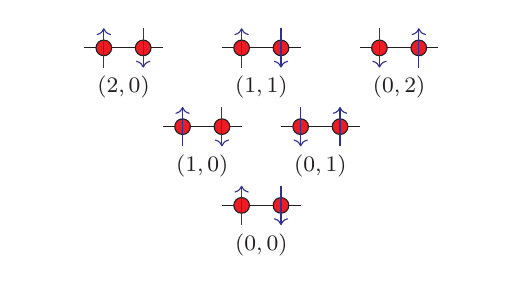
\begin{tikzpicture}[scale=0.5]
            \draw (-1,0) -- (1,0);
            \node at (-0.5,0) [draw,circle,fill=red,scale=0.6] {};
            \node at (0.5,0) [draw,circle,fill=red,scale=0.6] {};
            \draw[blue, ->] (-0.5,-0.5) -- (-0.5,0.5);
            \draw[blue, <-] (0.5,-0.5) -- (0.5,0.5);
            \node[text width=2.2cm, align=center] at (0,-1) {\footnotesize{$(0,0)$}};
            \draw (-2.5,2) -- (-0.5,2);
            \node at (-2.0,2) [draw,circle,fill=red,scale=0.6] {};
            \node at (-1.0,2) [draw,circle,fill=red,scale=0.6] {};
            \draw[blue, ->] (-2.0,1.5) -- (-2.0,2.5);
            \draw[blue, <-] (-1.0,1.5) -- (-1.0,2.5);
            \node[text width=2.2cm, align=center] at (-1.5,1) {\footnotesize{$(1,0)$}};
            \draw (0.5,2) -- (2.5,2);
            \node at (1.0,2) [draw,circle,fill=red,scale=0.6] {};
            \node at (2.0,2) [draw,circle,fill=red,scale=0.6] {};
            \draw[blue, <-] (1.0,1.5) -- (1.0,2.5);
            \draw[blue, ->] (2.0,1.5) -- (2.0,2.5);
            \node[text width=2.2cm, align=center] at (1.5,1) {\footnotesize{$(0,1)$}};
            \draw (-4.5,4) -- (-2.5,4);
            \node at (-4.0,4) [draw,circle,fill=red,scale=0.6] {};
            \node at (-3.0,4) [draw,circle,fill=red,scale=0.6] {};
            \draw[blue, ->] (-4.0,3.5) -- (-4.0,4.5);
            \draw[blue, <-] (-3.0,3.5) -- (-3.0,4.5);
            \node[text width=2.2cm, align=center] at (-3.5,3) {\footnotesize{$(2,0)$}};
            \draw (-1,4) -- (1,4);
            \node at (-0.5,4) [draw,circle,fill=red,scale=0.6] {};
            \node at (0.5,4) [draw,circle,fill=red,scale=0.6] {};
            \draw[blue, ->] (-0.5,3.5) -- (-0.5,4.5);
            \draw[blue, <-] (0.5,3.5) -- (0.5,4.5);
            \node[text width=2.2cm, align=center] at (0,3) {\footnotesize{$(1,1)$}};
            \draw (4.5,4) -- (2.5,4);
            \node at (4.0,4) [draw,circle,fill=red,scale=0.6] {};
            \node at (3.0,4) [draw,circle,fill=red,scale=0.6] {};
            \draw[blue, ->] (4.0,3.5) -- (4.0,4.5);
            \draw[blue, <-] (3.0,3.5) -- (3.0,4.5);
            \node[text width=2.2cm, align=center] at (3.5,3) {\footnotesize{$(0,2)$}};
        \end{tikzpicture}
    \end{figure}}
\end{frame}

\begin{frame}[fragile]{Methods: Hartree-Fock}
    \begin{itemize}[<+->]
        \item Constrained minimization
            \begin{itemize}
                \item Spin orthogonality: $\braket{\psi_i}{\psi_j} =
                    \delta_{ij}$
                \item Lagrange Multiplier method
                \item Fock-operator: $\mathcal{F} \equiv \mathcal{H}_0 + \mathcal{J} \pm \mathcal{K}$
                    \begin{itemize}[<4->]
                        \item $\mathcal{J} \equiv
                            \bra{\psi^{*}_k}f_{12}\ket{\psi_k} = \int
                            \psi^{*}_k(\blds{r})f_{12}\psi_k(\blds{r})\md r$
                        \vsp
                        \item $\mathcal{K} \equiv
                            \bra{\psi^{*}_k}f_{12}\ket{\psi} = \int
                            \psi^{*}_k(\blds{r})f_{12}\psi(\blds{r})\md r$
                        \vsp
                        \item<5-> \color{red}{$\mathcal{F}\ket{\psi} =
                            \blds{\veps}\ket{\psi},
                            \blds{\veps}=(\veps_0,\dots,\veps_N)$}
                    \end{itemize}
            \end{itemize}
    \end{itemize}
\end{frame}

{\setbeamercolor{palette primary}{fg=black, bg=white}
\begin{frame}[standout]
    $\mathcal{F}\ket{\psi} = \blds{\veps}\ket{\psi},\hspace{0.5cm}
    \blds{\veps}=(\veps_0,\dots,\veps_N)$
\end{frame}}

\begin{frame}[fragile]{Methods: Hartree-Fock}
    \begin{itemize}[<+->]
        \item Integrate out spin
        \item Pair spins as: $\{\psi_{2l-1}, \psi_{2l}\} =
            \{\phi_l(\blds{r})\alpha(s),\phi_l(\blds{r})\beta(s)\}$
        \item Expand: $\phi_i(\blds{r}) = \sum\limits^L_{p=1} C_{pi}\chi_p(\blds{r})$
        \item Roothan-Hall: $\blds{F}\blds{C}_i = \blds{\veps}S\blds{C}_i$
            \begin{itemize}[<4->]
                \item $F_{pq} = h_{pq} + \sum\limits_{pq}\rho_{pq}\left(2D_{prqs} \pm D_{prsq}\right)$
                \vsp
                \item $h_{pq} \equiv \Braket{p | h | q}$
                \vsp
                \item $\rho_{pq} \equiv \sum\limits^{\frac{N}{2}}_{i=1} C_{pi}C^{*}_{qi}$
                \vsp
                \item $D_{pqrs} \equiv \Braket{pq | f_{12} | rs}$
                \item $S_{pq} \equiv \Braket{p | q}$
            \end{itemize}
        \item Poople-Nesbet: $\blds{F}^{+}\blds{C}^{+} =
            \blds{\veps}^{\+}\blds{S}\blds{C}^{+}$, $\blds{F}^{-}\blds{C}^{-} =
            \blds{\veps}^{-}\blds{S}\blds{C}^{-}$
            \begin{itemize}[<5->]
                \item $F^{\pm}_{pq} = h_{pq} + \sumll{k_{\pm}}\sumll{rs}
                    C^{\pm\dagger}_{rk_{\pm}} C^{\pm\dagger}_{sk_{\pm}}
                    \left[D_{prqs} - D_{prsq}\right] +
                    \sumll{k_{\mp}}\sumll{rs} C^{\mp\dagger}_{rk_{\mp}}
                    C^{\mp\dagger}_{sk_{\mp}} D_{prqs}$
            \end{itemize}
    \end{itemize}
\end{frame}

\begin{frame}[fragile]{Methods: Hartree-Fock}
        \begin{figure}
            \centering
            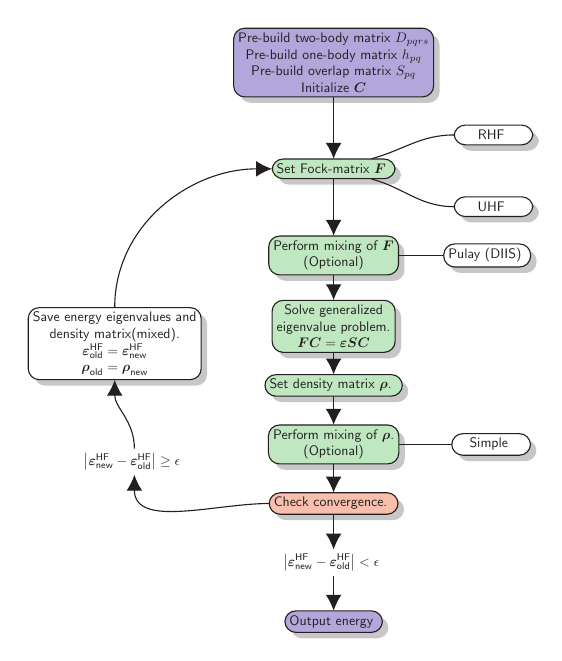
\begin{tikzpicture}[
                >={Latex[width=2mm,length=2mm]},
                    base/.style = {rectangle, rounded corners, draw=black,
                                minimum width=2cm, minimum height=0.5cm, text
                                centered, font=\sffamily},
                    basecode/.style = {rectangle, rounded corners, draw=black,
                                minimum width=2cm, minimum height=0.5cm, text
                                centered, font=\sffamily, align=left},
                    activityStarts/.style = {base, fill=blue!30, drop shadow},
                    startstop/.style = {base, fill=red!25, drop shadow},
                    startstopcode/.style = {basecode, fill=red!25, drop shadow},
                    activityRuns/.style = {base, fill=green!25, drop shadow},
                    process/.style = {base, fill=white!15, font=\sffamily, drop shadow},
                    processcode/.style = {basecode, fill=white!15, font=\sffamily, drop shadow},
                scale=0.5, 
                node distance=1.5cm, 
                every node/.style={fill=white, font=\sffamily, scale=0.5},
                align=center]
                \node (pre) [activityStarts] {
                    Pre-build two-body matrix $D_{pqrs}$ \\
                    Pre-build one-body matrix $h_{pq}$ \\
                    Pre-build overlap matrix $S_{pq}$ \\
                    Initialize $\blds{C}$
                };
                \node (Fock) [activityRuns, below of=pre, yshift=-1.2cm] {
                    Set Fock-matrix $\blds{F}$
                };
                \node (Fockmix) [activityRuns, below of=Fock, yshift=-0.7cm] {
                    Perform mixing of $\blds{F}$ \\
                    (Optional)
                };
                \node (Fockmixeq) [process, right of=Fockmix, xshift=2.4cm] {
                    Pulay (DIIS)
                };
                \draw[->] (Fock) -- (Fockmix);
                \draw[-] (Fockmix) -- (Fockmixeq);
                \node (RHF) [process, above right of=Fock, xshift=3.0cm, yshift=-0.2cm] {
                    RHF
                };
                \node (UHF) [process, below right of=Fock, xshift=3.0cm, yshift=0.1cm] {
                    UHF
                };
                \draw[-] (Fock) to [out=15, in=180] (RHF);
                \draw[-] (Fock) to [out=-15, in=180] (UHF);
                \draw[->] (pre) -- (Fock);
                \node (eigcomp) [activityRuns, below of=Fock, yshift=-2.5cm] {
                    Solve generalized \\ 
                    eigenvalue problem. \\
                    $\blds{F}\blds{C} = \blds{\veps}\blds{S}\blds{C}$
                };
                \draw[->] (Fockmix) -- (eigcomp);
                \node (density) [activityRuns, below of=eigcomp] {
                   Set density matrix $\blds{\rho}$.
                };
                \draw[->] (eigcomp) -- (density);
                \node (mix) [activityRuns, below of=density] {
                    Perform mixing of $\blds{\rho}$. \\
                    (Optional)
                };
                \draw[->] (density) -- (mix);
                \node (mixeq) [process, right of=mix, xshift=2.5cm] {
                    Simple
                };
                \draw[-] (mix) -- (mixeq);
                \node (conv) [startstop, below of=mix] {
                    Check convergence.
                };
                \draw[->] (mix) -- (conv);
                \node (no) [above left of=conv, xshift=-4.0cm] {
                    $\abs{\blds{\varepsilon}^{\text{HF}}_{\text{new}} -
                    \blds{\varepsilon}^{\text{HF}}_{\text{old}}} \geq \epsilon$
                };
                \draw[->] (conv) to [out=180,in=-90] (no);
                \node (keepOld) [process, above of=no, yshift=1.5cm, xshift=-0.5cm] {
                    Save energy eigenvalues and \\
                    density matrix(mixed). \\
                    $\blds{\varepsilon}^{\text{HF}}_{\text{old}} =
                    \blds{\varepsilon}^{\text{HF}}_{\text{new}}$ \\
                    $\blds{\rho}_{\text{old}} = \blds{\rho}_{\text{new}}$
                };
                \draw[->] (no) to [out=90,in=-90] (keepOld);
                \draw[->] (keepOld) to [out=90,in=180] (Fock);
                \node (yes) [below of=conv] {
                    $\abs{\blds{\varepsilon}^{\text{HF}}_{\text{new}} -
                    \blds{\varepsilon}^{\text{HF}}_{\text{old}}} < \epsilon$
                };
                \draw[->] (conv) -- (yes);
                \node (end) [activityStarts, below of=yes] {
                    Output energy
                };
                \draw[->] (yes) -- (end);
            \end{tikzpicture}
        \end{figure}
\end{frame}

{\setbeamercolor{palette primary}{fg=orange, bg=white}
\begin{frame}[standout]
    Variational Monte-Carlo
\end{frame}}

\begin{frame}[fragile]{Methods: Variational Monte-Carlo}
    \begin{itemize}[<+->]
        \item Variational Principle
        \item Rewrite expectation value:
            $\frac{\Braket{\Psi|\mathcal{H}|\Psi}}{\Braket{\Psi|\Psi}} = \int
            \frac{\cnj{\Psi}\mathcal{H}\Psi}{\int \cnj{\Psi}\Psi \md r} \md r
            = \int \frac{\abs{\Psi}^2E_L}{\int \cnj{\Psi}\Psi \md r} \md r$
            \begin{itemize}
                \item $E_L(\mb{R};\mb{\alpha}) \equiv \frac{1}{\Psi}\mathcal{H}\Psi$
                \item $P(\mb{R}) \equiv \frac{\abs{\Psi}^2}{\Braket{\Psi|\Psi}}$
            \end{itemize}
        \item Metropolis-Hastings Algorithm
            \begin{itemize}
                \item $r^{\text{new}} = r^{\text{old}} + \Delta t \xi$
                \item $\ufij{A}{i}{j} =
                    \text{min}\left(\frac{\ufij{P}{i}{j}}{\ufij{P}{j}{i}}
                    \frac{\ufij{T}{i}{j}}{\ufij{T}{j}{i}} ,1\right)$
                \item Importance Sampling
                    \begin{itemize}[<8->]
                        \item $r^{\text{new}} = r^{\text{old}} + D \Delta t
                            F^{\text{old}} + \sqrt{\Delta t}\xi$
                        \item $F = \frac{2}{\Psi}\nabla \Psi$ 
                        \item $\frac{T(b,a,\Delta t)}{T(a,b,\Delta t)} =
                            \sum\limits_i \exp(-\frac{\left(\blds{r}^{(b)}_i -
                            \blds{r}^{(a)}_i - D\Delta t
                            \blds{F}^{(a)}_i\right)^2}{4D\Delta t}
                            +\frac{\left(\blds{r}^{(a)}_i - \blds{r}^{(b)}_i -
                            D\Delta t \blds{F}^{(b)}_i\right)^2}{4D\Delta t})$
                    \end{itemize}
            \end{itemize}
    \end{itemize}
\end{frame}

\begin{frame}[fragile]{Methods: Variational Monte-Carlo}
    \begin{figure}[H]
        \centering
        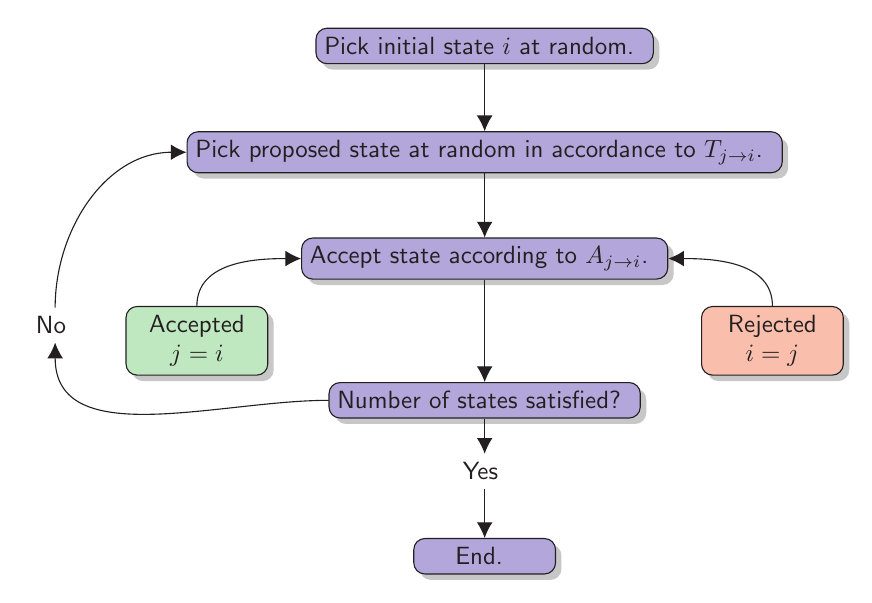
\begin{tikzpicture}[
            >={Latex[width=2mm,length=2mm]},
                base/.style = {rectangle, rounded corners, draw=black,
                            minimum width=2cm, minimum height=0.5cm, text
                            centered, font=\sffamily},
                basecode/.style = {rectangle, rounded corners, draw=black,
                            minimum width=2cm, minimum height=0.5cm, text
                            centered, font=\sffamily, align=left},
                activityStarts/.style = {base, fill=blue!30, drop shadow},
                startstop/.style = {base, fill=red!25, drop shadow},
                startstopcode/.style = {basecode, fill=red!25, drop shadow},
                activityRuns/.style = {base, fill=green!25, drop shadow},
                process/.style = {base, fill=white!15, font=\sffamily, drop shadow},
                processcode/.style = {basecode, fill=white!15, font=\sffamily, drop shadow},
            scale=0.8, 
            node distance=1.5cm, 
            every node/.style={fill=white, font=\sffamily, scale=0.9},
            align=center]
            \node (1) [activityStarts] {
                Pick initial state $i$ at random.
            };
            \node (2) [activityStarts, below of=1] {
                Pick proposed state at random in accordance to
                $\ufij{T}{j}{i}$.
            };
            \node (3) [activityStarts, below of=2] {
                Accept state according to $\ufij{A}{j}{i}$.
            };
            \node (a) [activityRuns, below left of=3, xshift=-3cm, yshift=-0.1cm] {
                Accepted \\
                $j = i$
            };
            \node (r) [startstop, below right of=3, xshift=3cm, yshift=-0.1cm] {
                Rejected \\
                $i = j$
            };
            \draw[<-] (3) to [out=180,in=90] (a);
            \draw[<-] (3) to [out=0,in=90] (r);
            \node (4) [activityStarts, below of=3, yshift=-0.5cm] {
                Number of states satisfied?
            };
            \node (yes) [below of=4, yshift=0.5cm] {
                Yes
            };
            \node (no) [above left of=4, xshift=-5cm] {
                No
            };
            \draw[->] (4) to [out=180, in=-90] (no);
            \draw[->] (no) to [out=90, in=180] (2);
            \node (5) [activityStarts, below of=yes, yshift=0.3cm] {
                End.
            };
            \draw[->] (1) -- (2);
            \draw[->] (2) -- (3);
            \draw[->] (3) -- (4);
            \draw[->] (4) -- (yes);
            \draw[->] (yes) -- (5);
        \end{tikzpicture}
    \end{figure}
\end{frame}

{\setbeamercolor{palette primary}{fg=orange, bg=white}
\begin{frame}[standout]
    Minimization
\end{frame}}

{\setbeamercolor{palette primary}{fg=black, bg=white}
\begin{frame}[standout]
    Single-Well\hspace{2cm} Rosenbrock
    \twofigure{text/figs/sphere.pdf}{text/figs/rosenbrock.pdf}
\end{frame}}

\begin{frame}[fragile]{Minimization: Gradient Descent}
    \begin{figure}[H]
        \centering
        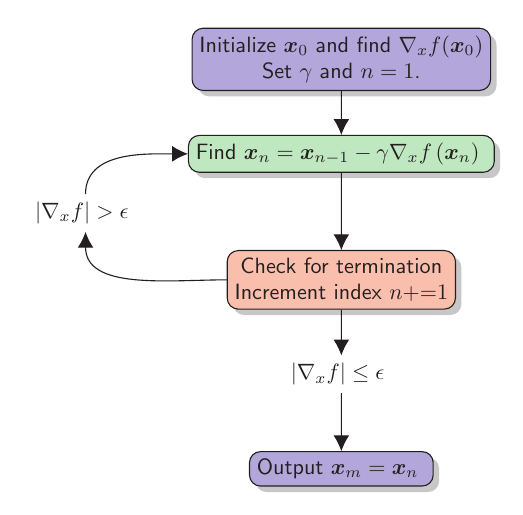
\begin{tikzpicture}[
                >={Latex[width=2mm,length=2mm]},
                    base/.style = {rectangle, rounded corners, draw=black,
                                minimum width=2cm, minimum height=0.5cm, text
                                centered, font=\sffamily},
                    basecode/.style = {rectangle, rounded corners, draw=black,
                                minimum width=2cm, minimum height=0.5cm, text
                                centered, font=\sffamily, align=left},
                    activityStarts/.style = {base, fill=blue!30, drop shadow},
                    startstop/.style = {base, fill=red!25, drop shadow},
                    startstopcode/.style = {basecode, fill=red!25, drop shadow},
                    activityRuns/.style = {base, fill=green!25, drop shadow},
                    process/.style = {base, fill=white!15, font=\sffamily, drop shadow},
                    processcode/.style = {basecode, fill=white!15, font=\sffamily, drop shadow},
                scale=0.8, 
                node distance=1.5cm, 
                every node/.style={fill=white, font=\sffamily, scale=0.8},
                align=center]
            \node (start) [activityStarts] {
                Initialize $\blds{x}_0$ and find
                $\nabla_{x}f({\blds{x}_0})$ \\
                Set $\gamma$ and $n=1$.
            };
            \node (update) [activityRuns, below of=start] {
                Find $\blds{x}_{n} = \blds{x}_{n-1} - \gamma
                \nabla_{x} f\left(\blds{x}_n\right)$
            };
            \draw[->] (start) -- (update);
            \node (conv) [startstop, below of=update, yshift=-0.5cm] {
                Check for termination \\
                Increment index $n {\footnotesize\mathrel{+}=} 1$
            };
            \draw[->] (update) -- (conv);
            \node (no) [above left of=conv, xshift=-3.0cm] {
                $\abs{\nabla_{x} f} > \epsilon$
            };
            \draw[->] (conv) to [out=180, in=-90] (no);
            \draw[->] (no) to [out=90, in=180] (update);
            \node (yes) [below of=conv] {
                $\abs{\nabla_{x} f} \leq \epsilon$
            };
            \draw[->] (conv) -- (yes);
            \node (end) [activityStarts, below of=yes] {
                Output $\blds{x}_m=\blds{x}_n$
            };
            \draw[->] (yes) -- (end);
        \end{tikzpicture}
    \end{figure}
\end{frame}

\begin{frame}[fragile]{Minimization: Gradient Descent}
    \vspace{-0.25cm}
    \begin{table}[H]
        \centering
        \footnotesize
        \setlength{\tabcolsep}{6.0pt}
        \begin{tabular}{ccccc} \hline\hline
            $\blds{x}_0$ & $\gamma$ & \color<2->{red}{Iterations} & $\blds{x}_m$ & $f(\blds{x}_m)$ \vsp \\
            $(5,5)$ & $0.9$ & $\color<2->{red}{20}$ & $(-0.072,-0.072)$ & $0.010$ \\
            $(5,5)$ & $0.9$ & $\color<2->{red}{50}$ & $(-8.920\times10^{-5},-8.920\times10^{-5})$ & $1.591\times10^{-8}$ \\
            $(5,5)$ & $0.9$ & $\color<2->{red}{100}$ & $(-1.273\times10^{-9},-1.273\times10^{-9})$ & $3.242\times10^{-18}$ \\
            $(5,5)$ & $0.5$ & $\color<2->{red}{20}$ & $(0.0,0.0)$ & $0.0$ \\
            $(5,5)$ & $0.5$ & $\color<2->{red}{50}$ & $(0.0,0.0)$ & $0.0$ \\
            $(5,5)$ & $0.5$ & $\color<2->{red}{100}$ & $(0.0,0.0)$ & $0.0$ \\
            $(5,5)$ & $0.1$ & $\color<2->{red}{20}$ & $(0.072,0.072)$ & $0.010$ \\
            $(5,5)$ & $0.1$ & $\color<2->{red}{50}$ & $(8.920\times10^{-5},8.920\times10^{-5})$ & $1.591\times10^{-8}$ \\
            $(5,5)$ & $0.1$ & $\color<2->{red}{100}$ & $(1.273\times10^{-9},1.273\times10^{-9})$ & $3.242\times10^{-18}$ \\ \hline\hline
        \end{tabular}
    \end{table}
    \vspace{-0.5cm}
    \begin{table}[H]
        \centering
        \footnotesize
        \setlength{\tabcolsep}{10.3pt}
        \begin{tabular}{ccccc} \hline\hline
            $\blds{x}_0$ & $\gamma$ & \color<2->{red}{Iterations} & $\blds{x}_m$ & $f(\blds{x}_m)$ \vsp \\
            $(0,0.5)$ & $0.001$ & $\color<2->{red}{100}$ & $(0.181,0.030)$ & $0.034$ \\
            $(0,0.5)$ & $0.001$ & $\color<2->{red}{500}$ & $(0.512,0.258)$ & $0.327$ \\
            $(0,0.5)$ & $0.001$ & $\color<2->{red}{1000}$ & $(0.675,0.454)$ & $0.106$ \\
            $(0,0.5)$ & $0.001$ & $\color<2->{red}{100000}$ & $(1.000,1.000) $ & $0.0$ \\
            $(0,0.5)$ & $0.0001$ & $\color<2->{red}{100}$ & $(0.027,0.068)$ & $1.399$ \\
            $(0,0.5)$ & $0.0001$ & $\color<2->{red}{500}$ & $(0.105,0.009)$ & $0.801$ \\
            $(0,0.5)$ & $0.0001$ & $\color<2->{red}{1000}$ & $(0.184,0.031)$ & $0.666$ \\
            $(0,0.5)$ & $0.0001$ & $\color<2->{red}{100000}$ & $(0.994,0.989)$ & $3.131\times10^{-5}$ \\ \hline\hline
        \end{tabular}
    \end{table}
\end{frame}

\begin{frame}[fragile]{Minimization: Quasi-Newton BFGS}
    \begin{figure}[H]
        \centering
        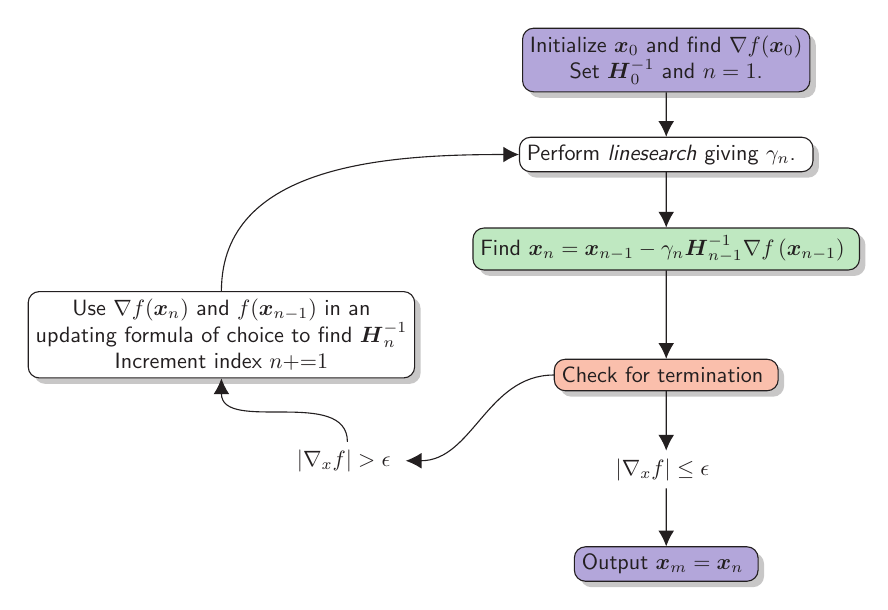
\begin{tikzpicture}[
                >={Latex[width=2mm,length=2mm]},
                    base/.style = {rectangle, rounded corners, draw=black,
                                minimum width=2cm, minimum height=0.5cm, text
                                centered, font=\sffamily},
                    basecode/.style = {rectangle, rounded corners, draw=black,
                                minimum width=2cm, minimum height=0.5cm, text
                                centered, font=\sffamily, align=left},
                    activityStarts/.style = {base, fill=blue!30, drop shadow},
                    startstop/.style = {base, fill=red!25, drop shadow},
                    startstopcode/.style = {basecode, fill=red!25, drop shadow},
                    activityRuns/.style = {base, fill=green!25, drop shadow},
                    process/.style = {base, fill=white!15, font=\sffamily, drop shadow},
                    processcode/.style = {basecode, fill=white!15, font=\sffamily, drop shadow},
                scale=0.8, 
                node distance=1.5cm, 
                every node/.style={fill=white, font=\sffamily, scale=0.8},
                align=center]
            \node (start) [activityStarts] {
                Initialize $\blds{x}_0$ and find $\nabla f({\blds{x}_0})$ \\
                Set $\blds{H}^{-1}_0$ and $n=1$.
            };
            \node (LS) [process, below of=start] {
                Perform \txtit{linesearch} giving $\gamma_n$.
            };
            \node (update) [activityRuns, below of=LS] {
                Find $\blds{x}_{n} = \blds{x}_{n-1} - \gamma_n
                \blds{H}^{-1}_{n-1}\nabla f\left(\blds{x}_{n-1}\right)$
            };
            \draw[->] (start) -- (LS);
            \draw[->] (LS) -- (update);
            \node (conv) [startstop, below of=update, yshift=-0.5cm] {
                Check for termination
            };
            \draw[->] (update) -- (conv);
            \node (no) [below left of=conv, xshift=-4.0cm, yshift=-0.3cm] {
                $\abs{\nabla_{x} f} > \epsilon$
            };
            \node (hupdate) [process, above of=no, xshift=-2.0cm, yshift=0.5cm] {
                Use $\nabla f(\blds{x}_n)$ and $f(\blds{x}_{n-1})$ in an \\
                updating formula of choice to find $\blds{H}^{-1}_n$ \\
                Increment index $n {\footnotesize\mathrel{+}=} 1$
            };
            \draw[->] (conv) to [out=180, in=0] (no);
            \draw[->] (no) to [out=90, in=-90] (hupdate);
            \draw[->] (hupdate) to [out=90, in=180] (LS);
            \node (yes) [below of=conv] {
                $\abs{\nabla_{x} f} \leq \epsilon$
            };
            \draw[->] (conv) -- (yes);
            \node (end) [activityStarts, below of=yes] {
                Output $\blds{x}_m=\blds{x}_n$
            };
            \draw[->] (yes) -- (end);
        \end{tikzpicture}
    \end{figure}
\end{frame}

\begin{frame}[fragile]{Minimization: Quasi-Newton BFGS}
    \vspace{-0.25cm}
    \begin{table}[H]
        \centering
        \footnotesize
        \setlength{\tabcolsep}{16.2pt}
        \begin{tabular}{cccc} \hline\hline
            $\blds{x}_0$ & \color<2->{red}{Iterations} & $\blds{x}_m$ & $f(\blds{x}_m)$ \vsp \\
            $(1,1)$ & $\color<2->{red}{1}$ & $(-0.071,-0.071)$ & $1.000$ \\
            $(-1,2)$ & $\color<2->{red}{1}$ & $(0.447,-0.894)$ & $1.000$ \\
            $(1,1)$ & $\color<2->{red}{2}$ & $(0.000,0.000)$ & $0.000$ \\
            $(-1,2)$ & $\color<2->{red}{2}$ & $(0.000,0.000)$ & $0.000$ \\
            $(10,10)$ & $\color<2->{red}{1}$ & $(-0.071,-0.071)$ & $1.000$ \\
            $(10,10)$ & $\color<2->{red}{2}$ & $(0.000,0.000)$ & $0.000$ \\
            $(100,100)$ & $\color<2->{red}{1}$ & $(-0.071,-0.071)$ & $1.000$ \\
            $(100,100)$ & $\color<2->{red}{2}$ & $(0.000,0.000)$ & $0.000$ \\ \hline\hline
        \end{tabular}
    \end{table}
    \vspace{-0.3cm}
    \begin{table}[H]
        \centering
        \footnotesize
        \setlength{\tabcolsep}{16.3pt}
        \begin{tabular}{ccccc} \hline\hline
            $\blds{x}_0$ & \color<2->{red}{Iterations} & $\blds{x}_m$ & $f(\blds{x}_m)$ \vsp \\
            $(-0.5,2.0)$ & $\color<2->{red}{1}$ & $(-0.706,0.708)$ & $7.280$ \\
            $(-0.5,2.0)$ & $\color<2->{red}{2}$ & $(-0.780,0.649)$ & $3.342$ \\
            $(-0.5,2.0)$ & $\color<2->{red}{10}$ & $(0.238,0.051)$ & $0.584$ \\
            $(-0.5,2.0)$ & $\color<2->{red}{30}$ & $(1.000,1,000)$ & $0.000$ \\
            $(5.5,-10.0)$ & $\color<2->{red}{1}$ & $(-0.996,0.091)$ & $85.214$ \\
            $(5.5,-10.0)$ & $\color<2->{red}{2}$ & $(-0.908,1.087)$ & $10.549$ \\
            $(5.5,-10.0)$ & $\color<2->{red}{10}$ & $(0.027,0.012)$ & $0.9613$ \\
            $(5.5,-10.0)$ & $\color<2->{red}{30}$ & $(1.000,1,000)$ & $0.000$ \\ \hline\hline
        \end{tabular}
    \end{table}
\end{frame}

% {\setbeamercolor{palette primary}{fg=black, bg=white}
% \begin{frame}[standout]{Minimization: Simulated Annealing}
%     \transduration<1->{0.}
%     \multiinclude[<+->][format=png, graphics={scale=0.5}, start=0]{text/sianData/fig}
% \end{frame}}

{\setbeamercolor{palette primary}{fg=black, bg=white}
\begin{frame}[standout]{Minimization: Simulated Annealing}
    \animategraphics[autoplay, controls, scale=0.5]{10}{text/sianData/fig-}{1}{99}
\end{frame}}

{\setbeamercolor{palette primary}{fg=black, bg=white}
\begin{frame}[standout]{Minimization: Simulated Annealing}
    Ackley\hspace{3cm} Rastrigin
    \twofigure{text/figs/ackley.pdf}{text/figs/rastrigin.pdf}
\end{frame}}

\section{Wavefunction}

{\setbeamercolor{palette primary}{fg=black, bg=white}
\begin{frame}[standout]{Wavefunction}
    \only<1->{$\phi_i(\blds{r}) = \sum\limits^L_{p=1} C_{pi}\chi_p(\blds{r})$}
    \only<2->{$\phi_i(\blds{r}) = \sum\limits^L_{p=1} C_{pi}\color{red}{\chi_p(\blds{r})}$}
\end{frame}}

{\setbeamercolor{palette primary}{fg=black, bg=white}
\begin{frame}[standout]{Wavefunction: Integral Elements}
    $\Braket{\phi_i(\blds{r})|\phi_j(\blds{r})}$ \\ \vsp\vsp\vsp\vsp
    $\Braket{\phi_i(\blds{r})|x^k_d|\phi_j(\blds{r})}$ \\ \vsp\vsp\vsp\vsp
    $\Braket{\phi_i(\blds{r})|\nabla^2|\phi_j(\blds{r})}$ \\ \vsp\vsp\vsp\vsp
    $\Braket{\phi_i(\blds{r}_1)\phi_j(\blds{r}_2)|f_{12}|\phi_k(\blds{r}_1)\phi_l(\blds{r}_2)}$ \\
\end{frame}}

\begin{frame}[fragile]{Wavefunction: Single-Well}
    \begin{itemize}[<+->]
        \item Hermite Function: $\psi_n(\blds{r}) \equiv \prod\limits_d N_d
            H_{n_d}(\sqrt{\omega}x_d)\exp(-\frac{\omega}{2}x^2_d)$
        \item Solution in polar\only<2->{\footfullcite{anisimovas}}
        \item $\psi_n(\blds{r}) = \prod\limits_d N_d \sum\limits^{n_d}_{l=1}
            C^{\text{Hermite}}_{n_dl}
            g_l\left(\frac{\omega}{2},\blds{r},\blds{0}\right)$
        \item Solution in Cartesian\only<4->{\footfullcite{HelgakerMolElcTheory}} \\ \vspace{0.2cm} \hspace{1cm}
            \begin{minipage}[H]{0.5\textwidth}
                $\Braket{g_i(\blds{r})|g_j(\blds{r})}$ \vsp \\
                $\Braket{g_i(\blds{r})|x^k_d|g_j(\blds{r})}$ \vsp \\
                $\Braket{g_i(\blds{r})|\nabla^2|g_j(\blds{r})}$ \vsp \\
                $\Braket{g_i(\blds{r}_1)g_j(\blds{r}_2)|f_{12}|g_k(\blds{r}_1)g_l(\blds{r}_2)}$ \\
            \end{minipage}
    \end{itemize}
\end{frame}

\begin{frame}[fragile]{Wavefunction: Single-Well Integral Elements}
    \centering\footnotesize
    $\Braket{\psiHO_i|\psiHO_j} = N_i \delta_{ij}$ \\
    $\Braket{\psiHO_i|h^{\text{HO}}|\psiHO_j} =
    N_i\varepsilon^{\text{HO}}_i\delta_{ij}$ \\
    $\Braket{\psiHO_i\psiHO_j|\frac{1}{r_{12}}|\psiHO_k\psiHO_l} =
    \frac{aN_{ijkl}}{\sqrt{2\omega}}  \sum\limits^{ijkl}_{tuvw} H^{ijkl}_{tuvw}
    \suml{pq}{t+v,u+w} E^{tv}_pE^{uw}_q (-1)^q\xi_{p+q}\left(\frac{\omega}{2},
    \blds{0}\right)$
        \begin{equation*}
            \begin{aligned}
                E^{i+1,j}_t &= \frac{1}{2(\alpha + \beta)}E^{ij}_{t-1} -
                \frac{\beta}{\alpha+\beta}(A_x - B_x)E^{ij}_t +
                (t+1)E^{ij}_{t+1} \\
                E^{i,j+1}_t &= \frac{1}{2(\alpha + \beta)}E^{ij}_{t-1} -
                \frac{\alpha}{\alpha+\beta}(A_y - B_y)E^{ij}_t +
                (t+1)E^{ij}_{t+1} \\
                E^{00}_0 &= K_{AB}
            \end{aligned}
        \end{equation*}
        \begin{equation*}
            \begin{aligned}
                \xi^n_{t+1,u} &= t\xi^{n+1}_{t-1,u} + X_{AB}\xi^{n+1}_{t,u} \\
                \xi^n_{t,u+1} &= u\xi^{n+1}_{t,u-1} + Y_{AB}\xi^{n+1}_{t,u} \\
                \xi^n_{00} &= \left(\frac{-2\alpha\beta}{\alpha+\beta}\right)^n
                \zeta_n\left(\frac{\alpha\beta}{\alpha+\beta} R^2_{AB}\right) \\
                \zeta_n(x) &= \int\limits^1_{-1} \frac{u^{2n}}{\sqrt{1 -
                u^2}} \me^{-u^2x} \md u
            \end{aligned} \hspace{0.5cm}
            \begin{aligned}
                \xi^n_{t+1,u,v} &= t\xi^{n+1}_{t-1,u,v} + X_{AB}\xi^{n+1}_{t,u,v} \\
                \xi^n_{t,u+1,v} &= u\xi^{n+1}_{t,u-1,v} + Y_{AB}\xi^{n+1}_{t,u,v} \\
                \xi^n_{t,u,v+1} &= u\xi^{n+1}_{t,u,v-1} + Y_{AB}\xi^{n+1}_{t,u,v} \\
                \xi^n_{000} &= \left(-2\alpha\beta\right)^n
                \zeta_n\left(\frac{\alpha\beta}{\alpha+\beta} R^2_{AB}\right)
                \\
                \zeta_n(x) &= \int\limits^1_{-1} u^{2n} \me^{-u^2x} \md u
            \end{aligned}
        \end{equation*}
\end{frame}

\begin{frame}[fragile]{Wavefunction: Double-Well}
    \begin{itemize}[<+->]
        \item Perturbation of harmonic oscillator: $\UDW(r) = \VHO(r) + \VDW_n(r)$
        \item Expand in HO-functions: $\ket{\psiDW_p} = \sumll{l}C^{\text{DW}}_{lp}\ket{\psiHO_l}$
        \item Eigenvalue equation: $\blds{H}^{\text{DW}}\blds{C}^{\text{DW}} =
            \blds{\varepsilon^{\text{DW}}}\blds{C}^{\text{DW}}$
            \begin{itemize}[<3->]
                \item $H^{\text{DW}}_{ij} = \veps^{\text{HO}}_i\delta_{ij} +
                    \Braket{\psiHO_i|\VDW_n|\psiHO_j}$
            \end{itemize}
        \item Integral-Elements
        \begin{equation*}
            \footnotesize
            \begin{aligned}
                \Braket{\psiDW_p|\psiDW_q} &= \delta_{pq} \\
                \Braket{\psiDW_p|h^{\text{DW}}|\psiDW_q} &=
                \varepsilon^{\text{DW}}_p\delta_{pq} \\
                \Braket{\psiDW_p\psiDW_q|\frac{1}{r_{12}}|\psiDW_r\psiDW_s} &=
                \suml{tuvw}{ijkl} C^{\text{DW}}_{tp}C^{\text{DW}}_{uq}C^{\text{DW}}_{vr}C^{\text{DW}}_{ws}
                \Braket{\psiHO_t\psiHO_u|\frac{1}{r_{12}}|\psiHO_v\psiHO_w}
            \end{aligned}
        \end{equation*}
    \end{itemize}
\end{frame}

\begin{frame}[fragile]{Wavefunction: Slater-Jastrow}
    \begin{itemize}[<+->]
        \item Slater determinant: $\psi_T =
            \det(\blds{\Phi(\blds{R};\blds{\alpha})}) \xi(s)$
        \item Modified Hermite: $\Phi_{ij} =
            \psi^{\text{HO}}_{n_j}(\sqrt{\alpha\omega}r_i) = \prod\limits_d N_d
            H_{n_d}(\sqrt{\alpha \omega}x_d)\me^{-\frac{\alpha\omega}{2}x^2_d}$
        \item Hartree-Fock: $\Phi_{ij} =
            \sum\limits_lC_{jl}\psi^{\text{HO}}_{n_l}\left(\sqrt{\omega}r_i\right)$
        \item Modified Hartree-Fock: $\Phi_{ij} =
            \sum\limits_lC_{jl}\psi^{\text{HO}}_{n_l}\left(\sqrt{\alpha\omega}r_i\right)$
        \item Pad\'e-Jastrow: $J_{\text{Pad\'e}} = \prod\limits_{i<j}
            \me^{\frac{a_{ij} r_{ij}}{1 + \beta r_{ij}}}$
        \item NQS: $J_{\text{NQS}} = \me^{-\suml{i=1}{N} \frac{\left(\bm{r}_i -
            \bm{a}_i\right)^2}{2\sigma^2}}\prod\limits^{M}_j \left(1 + \me^{b_j
            + \suml{i=1}{N}\suml{d=1}{D}
            \frac{x^{(d)}_iw_{i+d,j}}{\sigma^2}}\right)$
        \item Pad\'e-NQS: $J = J_{\text{Pad\'e}}J_{\text{NQS}}$
    \end{itemize}
\end{frame}

\section{Implementation}

\begin{frame}[fragile]{Implementation}
    \begin{itemize}[<+->]
        \item \CC and Eigen
            \begin{itemize}
                \item Performance
                \item Generalization
            \end{itemize}
        \item Python
            \begin{itemize}
               \item Generate \CC code 
            \end{itemize}
    \end{itemize}
\end{frame}

\begin{frame}[fragile]{Implementation: Cartesian}
    \begin{figure}[H]
        \centering
        \begin{tikzpicture}[scale=1.0]
            \draw (-1,0) -- (1,0);
            \node at (-0.5,0) [draw,circle,fill=red,scale=0.6] {};
            \node at (0.5,0) [draw,circle,fill=red,scale=0.6] {};
            \draw[blue, ->] (-0.5,-0.5) -- (-0.5,0.5);
            \draw[blue, <-] (0.5,-0.5) -- (0.5,0.5);
            \node[text width=2.2cm, align=center] at (0,-1) {\footnotesize{$(0,0)$}};
            \draw (-2.5,2) -- (-0.5,2);
            \node at (-2.0,2) [draw,circle,fill=red,scale=0.6] {};
            \node at (-1.0,2) [draw,circle,fill=red,scale=0.6] {};
            \draw[blue, ->] (-2.0,1.5) -- (-2.0,2.5);
            \draw[blue, <-] (-1.0,1.5) -- (-1.0,2.5);
            \node[text width=2.2cm, align=center] at (-1.5,1) {\footnotesize{$(1,0)$}};
            \draw (0.5,2) -- (2.5,2);
            \node at (1.0,2) [draw,circle,fill=red,scale=0.6] {};
            \node at (2.0,2) [draw,circle,fill=red,scale=0.6] {};
            \draw[blue, <-] (1.0,1.5) -- (1.0,2.5);
            \draw[blue, ->] (2.0,1.5) -- (2.0,2.5);
            \node[text width=2.2cm, align=center] at (1.5,1) {\footnotesize{$(0,1)$}};
            \draw (-4.5,4) -- (-2.5,4);
            \node at (-4.0,4) [draw,circle,fill=red,scale=0.6] {};
            \node at (-3.0,4) [draw,circle,fill=red,scale=0.6] {};
            \draw[blue, ->] (-4.0,3.5) -- (-4.0,4.5);
            \draw[blue, <-] (-3.0,3.5) -- (-3.0,4.5);
            \node[text width=2.2cm, align=center] at (-3.5,3) {\footnotesize{$(2,0)$}};
            \draw (-1,4) -- (1,4);
            \node at (-0.5,4) [draw,circle,fill=red,scale=0.6] {};
            \node at (0.5,4) [draw,circle,fill=red,scale=0.6] {};
            \draw[blue, ->] (-0.5,3.5) -- (-0.5,4.5);
            \draw[blue, <-] (0.5,3.5) -- (0.5,4.5);
            \node[text width=2.2cm, align=center] at (0,3) {\footnotesize{$(1,1)$}};
            \draw (4.5,4) -- (2.5,4);
            \node at (4.0,4) [draw,circle,fill=red,scale=0.6] {};
            \node at (3.0,4) [draw,circle,fill=red,scale=0.6] {};
            \draw[blue, ->] (4.0,3.5) -- (4.0,4.5);
            \draw[blue, <-] (3.0,3.5) -- (3.0,4.5);
            \node[text width=2.2cm, align=center] at (3.5,3) {\footnotesize{$(0,2)$}};
        \end{tikzpicture}
    \end{figure}
\end{frame}

\begin{frame}[fragile]{Implementation: Hartree-Fock}
    \only<1->{
    \begin{figure}[H]
        \centering
        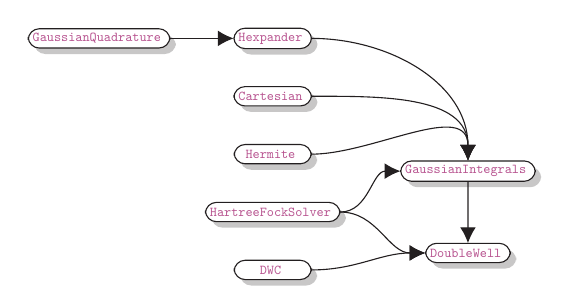
\begin{tikzpicture}[
            >={Latex[width=2mm,length=2mm]},
                base/.style = {rectangle, rounded corners, draw=black,
                            minimum width=2cm, minimum height=0.5cm, text
                            centered, font=\sffamily},
                basecode/.style = {rectangle, rounded corners, draw=black,
                            minimum width=2cm, minimum height=0.5cm, text
                            centered, font=\sffamily, align=left},
                activityStarts/.style = {base, fill=blue!30, drop shadow},
                startstop/.style = {base, fill=red!25, drop shadow},
                startstopcode/.style = {basecode, fill=red!25, drop shadow},
                activityRuns/.style = {base, fill=green!25, drop shadow},
                process/.style = {base, fill=white!15, font=\sffamily, drop shadow},
                processcode/.style = {basecode, fill=white!15, font=\sffamily, drop shadow},
            scale=0.8, 
            node distance=1.5cm, 
            every node/.style={fill=white, font=\sffamily, scale=0.49},
            align=center]
            \node (Hexpander) [processcode] {
                \hltexttt{Hexpander}
            };
            \node (GaussianQuadrature) [processcode, left of=Hexpander, xshift=-3cm] {
                \hltexttt{GaussianQuadrature}
            };
            \node (Cartesian) [processcode, below of=Hexpander] {
                \hltexttt{Cartesian}
            };
            \node (Hermite) [processcode, below of=Cartesian] {
                \hltexttt{Hermite}
            };
            \node (HartreeFockSolver) [processcode, below of=Hermite] {
                \hltexttt{HartreeFockSolver}
            };
            \node (GaussianIntegrals) [processcode, above right of=HartreeFockSolver, xshift=4cm] {
                \hltexttt{GaussianIntegrals}
            };
            \node (DoubleWell) [processcode, below right of=HartreeFockSolver, xshift=4cm] {
                \hltexttt{DoubleWell}
            };
            \node (DWC) [processcode, below of=HartreeFockSolver] {
                \hltexttt{DWC}
            };
            \draw[->] (GaussianQuadrature) -- (Hexpander);
            \draw[->] (Hexpander) to [out=0, in=90] (GaussianIntegrals);
            \draw[->] (Cartesian) to [out=0, in=90] (GaussianIntegrals);
            \draw[->] (Hermite) to [out=0, in=90] (GaussianIntegrals);
            \draw[->] (HartreeFockSolver) to [out=0, in=180] (GaussianIntegrals);
            \draw[->] (HartreeFockSolver) to [out=0, in=180] (DoubleWell);
            \draw[->] (DWC) to [out=0, in=180] (DoubleWell);
            \draw[->] (GaussianIntegrals) -- (DoubleWell);
        \end{tikzpicture}
    \end{figure}}
    \begin{itemize}
        \item<2-> Parallelization
            \begin{itemize}[<3->]
                \item Two-body element is computationally expensive
                \item $S_i = \suml{j=0}{P_i} \prod\limits_d (n_{j_d}+1)$
            \end{itemize}
        \item<4-> Hartree-Fock algorithm only run on one process
        \item<5-> Tabulation of Two-Body matrix
    \end{itemize}
\end{frame}

\begin{frame}[fragile]{Implementation: Variational Monte-Carlo}
    \only<1->{
    \begin{figure}[H]
        \centering
        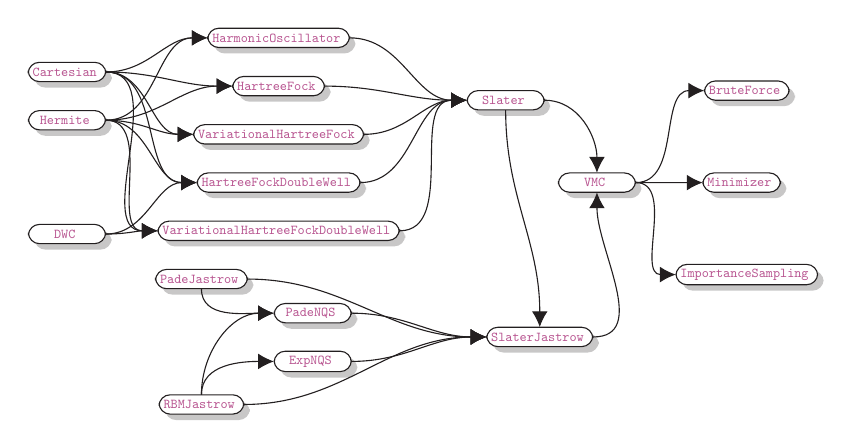
\begin{tikzpicture}[
            >={Latex[width=2mm,length=2mm]},
                base/.style = {rectangle, rounded corners, draw=black,
                            minimum width=2cm, minimum height=0.5cm, text
                            centered, font=\sffamily},
                basecode/.style = {rectangle, rounded corners, draw=black,
                            minimum width=2cm, minimum height=0.5cm, text
                            centered, font=\sffamily, align=left},
                activityStarts/.style = {base, fill=blue!30, drop shadow},
                startstop/.style = {base, fill=red!25, drop shadow},
                startstopcode/.style = {basecode, fill=red!25, drop shadow},
                activityRuns/.style = {base, fill=green!25, drop shadow},
                process/.style = {base, fill=white!15, font=\sffamily, drop shadow},
                processcode/.style = {basecode, fill=white!15, font=\sffamily, drop shadow},
            scale=0.8, 
            node distance=1.25cm, 
            every node/.style={fill=white, font=\sffamily, scale=0.49},
            align=center]
            \node (HarmonicOscillator) [processcode] {
                \hltexttt{HarmonicOscillator}
            };
            \node (HartreeFock) [processcode, below of=HarmonicOscillator] {
                \hltexttt{HartreeFock}
            };
            \node (VariationalHartreeFock) [processcode, below of=HartreeFock] {
                \hltexttt{VariationalHartreeFock}
            };
            \node (HartreeFockDoubleWell) [processcode, below of=VariationalHartreeFock] {
                \hltexttt{HartreeFockDoubleWell}
            };
            \node (VariationalHartreeFockDoubleWell) [processcode, below of=HartreeFockDoubleWell] {
                \hltexttt{VariationalHartreeFockDoubleWell}
            };
            \node (PadeJastrow) [processcode, below of=VariationalHartreeFockDoubleWell, xshift=-2cm] {
                \hltexttt{PadeJastrow}
            };
            \node (RBMJastrow) [processcode, below of=PadeJastrow, yshift=-2cm] {
                \hltexttt{RBMJastrow}
            };
            \node (PadeNQS) [processcode, below right of=PadeJastrow, xshift=2.0cm] {
                \hltexttt{PadeNQS}
            };
            \node (ExpNQS) [processcode, below of=PadeNQS] {
                \hltexttt{ExpNQS}
            };
            \node (Cartesian) [processcode, below left of=HarmonicOscillator, xshift=-4.6cm] {
                \hltexttt{Cartesian}
            };
            \node (Hermite) [processcode, below of=Cartesian] {
                \hltexttt{Hermite}
            };
            \node (DWC) [processcode, below of=Hermite, yshift=-1.7cm] {
                \hltexttt{DWC}
            };
            \node (Slater) [processcode, above right of=VariationalHartreeFock, xshift=5cm] {
                \hltexttt{Slater}
            };
            \node (SlaterJastrow) [processcode, above right of=PadeNQS, xshift=5cm, yshift=-1.5cm] {
                \hltexttt{SlaterJastrow}
            };
            \node (VMC) [processcode, right of=HartreeFockDoubleWell, xshift=7cm] {
                \hltexttt{VMC}
            };
            \node (Minimizer) [processcode, right of=VMC, xshift=2.5cm] {
                \hltexttt{Minimizer}
            };
            \node (BruteForce) [processcode, above right of=VMC, xshift=3cm, yshift=1.5cm] {
                \hltexttt{BruteForce}
            };
            \node (ImportanceSampling) [processcode, below right of=VMC, xshift=3cm, yshift=-1.5cm] {
                \hltexttt{ImportanceSampling}
            };
            \draw[->] (Cartesian) to [out=0, in=180] (HarmonicOscillator);
            \draw[->] (Cartesian) to [out=0, in=180] (HartreeFock);
            \draw[->] (Cartesian) to [out=0, in=180] (VariationalHartreeFock);
            \draw[->] (Cartesian) to [out=0, in=180] (HartreeFockDoubleWell);
            \draw[->] (Cartesian) to [out=0, in=180] (VariationalHartreeFockDoubleWell);
            \draw[->] (Hermite) to [out=0, in=180] (HarmonicOscillator);
            \draw[->] (Hermite) to [out=0, in=180] (HartreeFock);
            \draw[->] (Hermite) to [out=0, in=180] (VariationalHartreeFock);
            \draw[->] (Hermite) to [out=0, in=180] (HartreeFockDoubleWell);
            \draw[->] (Hermite) to [out=0, in=180] (VariationalHartreeFockDoubleWell);
            \draw[->] (DWC) to [out=0, in=180] (HartreeFockDoubleWell);
            \draw[->] (DWC) to [out=0, in=180] (VariationalHartreeFockDoubleWell);
            \draw[->]  (HarmonicOscillator)               to [out=0, in=180] (Slater);
            \draw[->]  (HartreeFock)                      to [out=0, in=180] (Slater);
            \draw[->]  (VariationalHartreeFock)           to [out=0, in=180] (Slater);
            \draw[->]  (HartreeFockDoubleWell)            to [out=0, in=180] (Slater);
            \draw[->]  (VariationalHartreeFockDoubleWell) to [out=0, in=180] (Slater);
            \draw[->]  (PadeJastrow)            to [out=0, in=180] (SlaterJastrow);
            \draw[->]  (RBMJastrow)                      to [out=0, in=180] (SlaterJastrow);
            \draw[->]  (PadeNQS)           to [out=0, in=180] (SlaterJastrow);
            \draw[->]  (ExpNQS)            to [out=0, in=180] (SlaterJastrow);
            \draw[->]  (Slater)            to [out=-90, in=90] (SlaterJastrow);
            \draw[->]  (Slater)            to [out=0, in=90] (VMC);
            \draw[->]  (SlaterJastrow)      to [out=0, in=-90] (VMC);
            \draw[->]  (VMC)    to [out=0, in=180] (BruteForce);
            \draw[->]  (VMC)    to [out=0, in=180] (ImportanceSampling);
            \draw[->]  (VMC)    to [out=0, in=180] (Minimizer);
            \draw[->]  (PadeJastrow)    to [out=-90, in=180] (PadeNQS);
            \draw[->]  (RBMJastrow)    to [out=90, in=180] (PadeNQS);
            \draw[->]  (RBMJastrow)    to [out=90, in=180] (ExpNQS);
        \end{tikzpicture}
    \end{figure}}
    \begin{itemize}[<2->]
        \item \hltexttt{Hermite} generated with Python and SymPy
    \end{itemize}
\end{frame}

\begin{frame}[fragile]{Implementation: Variational Monte-Carlo}
    \footnotesize
    \begin{itemize}
        \item {\makebox[3cm]{\hltextttf{set}:\hfill} Called during
            initialization (before each sampling)} \\
        \item {\makebox[3cm]{\hltextttf{reSetAll}:\hfill} Sets all matrices
            to zero (used in testing)} \\
        \item {\makebox[3cm]{\hltextttf{initializeMatrices}:\hfill}
            Allocate memory} \\
        \item {\makebox[3cm]{\hltextttf{update}:\hfill} Update positions
            and wavefunction} \\
        \item {\makebox[3cm]{\hltextttf{reset}:\hfill} Revert to previous
            positions and wavefunction} \\
        \item {\makebox[3cm]{\hltextttf{resetGradient}:\hfill} Revert to
            previous gradient} \\
        \item {\makebox[3cm]{\hltextttf{acceptState}:\hfill} Update
            previous positions and wavefunction to current} \\
        \item {\makebox[3cm]{\hltextttf{acceptGradient}:\hfill} Update
            previous gradient to current one}
    \end{itemize}
\end{frame}

\begin{frame}[fragile]{Implementation: Variational Monte-Carlo}
    \only<1->{
    \begin{figure}[H]
        \centering
        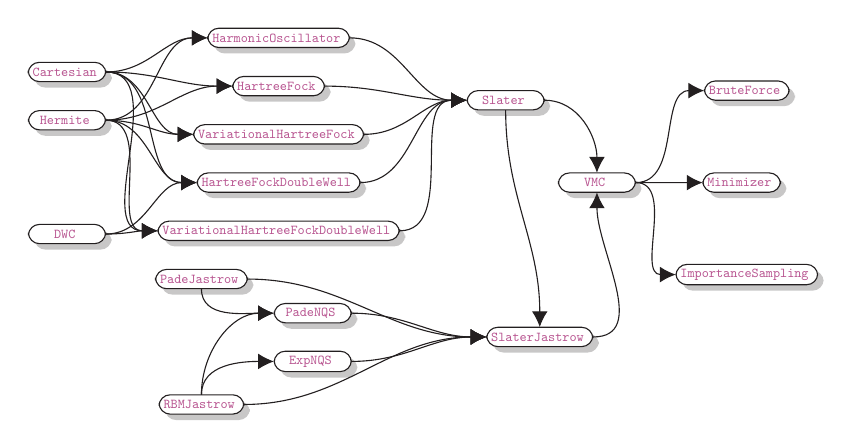
\begin{tikzpicture}[
            >={Latex[width=2mm,length=2mm]},
                base/.style = {rectangle, rounded corners, draw=black,
                            minimum width=2cm, minimum height=0.5cm, text
                            centered, font=\sffamily},
                basecode/.style = {rectangle, rounded corners, draw=black,
                            minimum width=2cm, minimum height=0.5cm, text
                            centered, font=\sffamily, align=left},
                activityStarts/.style = {base, fill=blue!30, drop shadow},
                startstop/.style = {base, fill=red!25, drop shadow},
                startstopcode/.style = {basecode, fill=red!25, drop shadow},
                activityRuns/.style = {base, fill=green!25, drop shadow},
                process/.style = {base, fill=white!15, font=\sffamily, drop shadow},
                processcode/.style = {basecode, fill=white!15, font=\sffamily, drop shadow},
            scale=0.8, 
            node distance=1.25cm, 
            every node/.style={fill=white, font=\sffamily, scale=0.49},
            align=center]
            \node (__HarmonicOscillator) [processcode] {
                \hltexttt{HarmonicOscillator}
            };
            \node (__HartreeFock) [processcode, below of=__HarmonicOscillator] {
                \hltexttt{HartreeFock}
            };
            \node (__VariationalHartreeFock) [processcode, below of=__HartreeFock] {
                \hltexttt{VariationalHartreeFock}
            };
            \node (__HartreeFockDoubleWell) [processcode, below of=__VariationalHartreeFock] {
                \hltexttt{HartreeFockDoubleWell}
            };
            \node (__VariationalHartreeFockDoubleWell) [processcode, below of=__HartreeFockDoubleWell] {
                \hltexttt{VariationalHartreeFockDoubleWell}
            };
            \node (__PadeJastrow) [processcode, below of=__VariationalHartreeFockDoubleWell, xshift=-2cm] {
                \hltexttt{PadeJastrow}
            };
            \node (__RBMJastrow) [processcode, below of=__PadeJastrow, yshift=-2cm] {
                \hltexttt{RBMJastrow}
            };
            \node (__PadeNQS) [processcode, below right of=__PadeJastrow, xshift=2.0cm] {
                \hltexttt{PadeNQS}
            };
            \node (__ExpNQS) [processcode, below of=__PadeNQS] {
                \hltexttt{ExpNQS}
            };
            \node (__Cartesian) [processcode, below left of=__HarmonicOscillator, xshift=-4.6cm] {
                \hltexttt{Cartesian}
            };
            \node (__Hermite) [processcode, below of=__Cartesian] {
                \hltexttt{Hermite}
            };
            \node (__DWC) [processcode, below of=__Hermite, yshift=-1.7cm] {
                \hltexttt{DWC}
            };
            \node (__Slater) [processcode, above right of=__VariationalHartreeFock, xshift=5cm] {
                \hltexttt{Slater}
            };
            \node (__SlaterJastrow) [processcode, above right of=__PadeNQS, xshift=5cm, yshift=-1.5cm] {
                \hltexttt{SlaterJastrow}
            };
            \node (__VMC) [processcode, right of=__HartreeFockDoubleWell, xshift=7cm] {
                \hltexttt{VMC}
            };
            \node (__Minimizer) [processcode, right of=__VMC, xshift=2.5cm] {
                \hltexttt{Minimizer}
            };
            \node (__BruteForce) [processcode, above right of=__VMC, xshift=3cm, yshift=1.5cm] {
                \hltexttt{BruteForce}
            };
            \node (__ImportanceSampling) [processcode, below right of=__VMC, xshift=3cm, yshift=-1.5cm] {
                \hltexttt{ImportanceSampling}
            };
            \draw[->] (__Cartesian) to [out=0, in=180] (__HarmonicOscillator);
            \draw[->] (__Cartesian) to [out=0, in=180] (__HartreeFock);
            \draw[->] (__Cartesian) to [out=0, in=180] (__VariationalHartreeFock);
            \draw[->] (__Cartesian) to [out=0, in=180] (__HartreeFockDoubleWell);
            \draw[->] (__Cartesian) to [out=0, in=180] (__VariationalHartreeFockDoubleWell);
            \draw[->] (__Hermite) to [out=0, in=180] (__HarmonicOscillator);
            \draw[->] (__Hermite) to [out=0, in=180] (__HartreeFock);
            \draw[->] (__Hermite) to [out=0, in=180] (__VariationalHartreeFock);
            \draw[->] (__Hermite) to [out=0, in=180] (__HartreeFockDoubleWell);
            \draw[->] (__Hermite) to [out=0, in=180] (__VariationalHartreeFockDoubleWell);
            \draw[->] (__DWC) to [out=0, in=180] (__HartreeFockDoubleWell);
            \draw[->] (__DWC) to [out=0, in=180] (__VariationalHartreeFockDoubleWell);
            \draw[->]  (__HarmonicOscillator)               to [out=0, in=180] (__Slater);
            \draw[->]  (__HartreeFock)                      to [out=0, in=180] (__Slater);
            \draw[->]  (__VariationalHartreeFock)           to [out=0, in=180] (__Slater);
            \draw[->]  (__HartreeFockDoubleWell)            to [out=0, in=180] (__Slater);
            \draw[->]  (__VariationalHartreeFockDoubleWell) to [out=0, in=180] (__Slater);
            \draw[->]  (__PadeJastrow)            to [out=0, in=180] (__SlaterJastrow);
            \draw[->]  (__RBMJastrow)                      to [out=0, in=180] (__SlaterJastrow);
            \draw[->]  (__PadeNQS)           to [out=0, in=180] (__SlaterJastrow);
            \draw[->]  (__ExpNQS)            to [out=0, in=180] (__SlaterJastrow);
            \draw[->]  (__Slater)            to [out=-90, in=90] (__SlaterJastrow);
            \draw[->]  (__Slater)            to [out=0, in=90] (__VMC);
            \draw[->]  (__SlaterJastrow)      to [out=0, in=-90] (__VMC);
            \draw[->]  (__VMC)    to [out=0, in=180] (__BruteForce);
            \draw[->]  (__VMC)    to [out=0, in=180] (__ImportanceSampling);
            \draw[->]  (__VMC)    to [out=0, in=180] (__Minimizer);
            \draw[->]  (__PadeJastrow)    to [out=-90, in=180] (__PadeNQS);
            \draw[->]  (__RBMJastrow)    to [out=90, in=180] (__PadeNQS);
            \draw[->]  (__RBMJastrow)    to [out=90, in=180] (__ExpNQS);
        \end{tikzpicture}
    \end{figure}}
    \begin{itemize}
        \item<1-> \hltexttt{Hermite} generated with Python and SymPy
        \item<2-> Wavefunction class can be created with Python
    \end{itemize}
\end{frame}

\section{Results}

{\setbeamercolor{palette primary}{fg=orange, bg=white}
\begin{frame}[standout]
    Benchmark
\end{frame}}

\begin{frame}[fragile]{Results: Benchmark}
    \vspace{-0.25cm}
    \twofigure{text/figs/N2.pdf}{text/figs/N6.pdf}
    \vspace{-0.5cm}
    \twofigure{text/figs/N12.pdf}{text/figs/N20.pdf}
\end{frame}

\begin{frame}[fragile]{Results: Benchmark}
    \vspace{-0.25cm}
    \twofigure{text/figs/N30.pdf}{text/figs/N42.pdf}
    \vspace{-0.5cm}
    \onefigure{text/figs/N56.pdf}
\end{frame}

\begin{frame}[fragile]{Results: Benchmark}
    \vspace{-0.25cm}
    \twofigure{text/figs/N2_D3.pdf}{text/figs/N8_D3.pdf}
    \vspace{-0.5cm}
    \twofigure{text/figs/N20_D3.pdf}{text/figs/N40_D3.pdf}
\end{frame}

\begin{frame}[fragile]{Results: Benchmark}
    \vspace{-0.25cm}
    \input{text/tables/tableHObench2D}
    \vspace{-0.7cm}
    \input{text/tables/tableHObench3D}
    \begin{equation*}
        \psi =
        \psi^{\text{HO}}\left(\sqrt{\alpha\omega}\right)J_{\text{Pad\'e}}
    \end{equation*}
\end{frame}

\begin{frame}[fragile]{Results: Benchmark}
    \vspace{-0.25cm}
    \input{text/tables/tHF2DVMCHO}
    \vspace{-0.5cm}
    \input{text/tables/tHFVAR2DVMCHO}
    \begin{equation*}
        \psi_p =
        \sum_lC_{lp}\psi^{\text{HO}}_l\left(\sqrt{\omega}r\right)J_{\text{Pad\'e}},\hspace{0.5cm}
        \psi_p =
        \sum_lC_{lp}\psi^{\text{HO}}_l\left(\sqrt{\alpha\omega}r\right)J_{\text{Pad\'e}}
    \end{equation*}
\end{frame}

\begin{frame}[fragile]{Results: Benchmark}
    \vspace{-0.25cm}
    \input{text/tables/tHF3DVMCHO}
    \vspace{-0.5cm}
    \input{text/tables/tHFVAR3DVMCHO}
    \begin{equation*}
        \psi_p =
        \sum_lC_{lp}\psi^{\text{HO}}_l\left(\sqrt{\omega}r\right)J_{\text{Pad\'e}},\hspace{0.5cm}
        \psi_p =
        \sum_lC_{lp}\psi^{\text{HO}}_l\left(\sqrt{\alpha\omega}r\right)J_{\text{Pad\'e}}
    \end{equation*}
\end{frame}

\begin{frame}[fragile]{Results: Double-Well Hartree-Fock}
    \onefigure{text/figs/D2_DW.pdf}
    \vspace{-0.8cm}
    \onefigure{text/figs/D3_DW.pdf}
\end{frame}

\begin{frame}[fragile]{Results: Double-Well Variational Monte-Carlo}
    \input{text/tables/tHF2DVMCDW}
    \begin{equation*}
        \psi_p =
        \sum_lC^{\text{HF}}_{lp}\sum_kC^{\text{DW}}_{kl}\psi^{\text{HO}}_k\left(\sqrt{\omega}r\right)J_{\text{Pad\'e}}
    \end{equation*}
    \input{text/tables/tHFVAR2DVMCDW}
    \begin{equation*}
        \psi_p =
        \sum_lC^{\text{HF}}_{lp}\sum_kC^{\text{DW}}_{kl}\psi^{\text{HO}}_k\left(\sqrt{\alpha\omega}r\right)J_{\text{Pad\'e}}
    \end{equation*}
\end{frame}

\begin{frame}[fragile]{Results: Double-Well Variational Monte-Carlo}
    \input{text/tables/tHF3DVMCDW}
    \begin{equation*}
        \psi_p =
        \sum_lC^{\text{HF}}_{lp}\sum_kC^{\text{DW}}_{kl}\psi^{\text{HO}}_k\left(\sqrt{\omega}r\right)J_{\text{Pad\'e}}
    \end{equation*}
    \input{text/tables/tHFVAR3DVMCDW}
    \begin{equation*}
        \psi_p =
        \sum_lC^{\text{HF}}_{lp}\sum_kC^{\text{DW}}_{kl}\psi^{\text{HO}}_k\left(\sqrt{\alpha\omega}r\right)J_{\text{Pad\'e}}
    \end{equation*}
\end{frame}

{\setbeamercolor{palette primary}{fg=black, bg=white}
\begin{frame}[standout]{Results: NQS-Jastrow}
    $J_{\text{NQS}} = \me^{-\suml{i=1}{N} \frac{\left({r}_i -
    {a}_i\right)^2}{2\sigma^2}}\prod\limits^{M}_j \left(1 + \me^{b_j +
    \suml{i=1}{N}\suml{d=1}{D} \frac{x^{(d)}_iw_{i+d,j}}{\sigma^2}}\right)$
\end{frame}}

\begin{frame}[fragile]{Results: NQS-Jastrow Harmonic Oscillator}
    \vspace{-0.26cm}
    \twofigure{{text/figs/w1.0_N2_D2_padenqs}.pdf}{{text/figs/w1.0_N6_D2_padenqs}.pdf}
    \vspace{-0.65cm}
    \twofigure{{text/figs/w1.0_D3_N2_energies_fig}.pdf}{{text/figs/w1.0_D3_N8_energies_fig}.pdf}
\end{frame}

\section{Summary and Conclusion}

{\setbeamercolor{palette primary}{fg=orange, bg=white}
\begin{frame}[standout]
  Questions?
\end{frame}}

\appendix

{\setbeamercolor{palette primary}{fg=orange, bg=white}
\begin{frame}[standout]{Questions}
    Questions?
\end{frame}}

\end{document}
